%%%%
\section{África}

A poluição do ar ambiental nas cidades dos países em desenvolvimento
guarda algumas similaridades com as cidades dos países desenvolvidos,
ambas possuem fontes poluidoras que são características de meios urbanos, 
tais como: tráfego de veículos automotivos, industrias, geração de 
eletricidade por usina hidrelétrica ou termoelétrica, entre outras. 

No entanto, em cidades de países de industrialização tardia, soma-se a esta 
poluição, comum a meios urbanos, agravantes decorrentes da incapacidade do 
Estado em atender toda a população nas demandas urbanas de infraestrutura. 
Entre as falhas do governo, destaca-se a omissão em prover energia 
necessária para realização de atividades cotidianas, como, transporte, 
moradia, iluminação e alimentação. 
A queima de biomassa para cozimento de alimentos, o uso de querosene para 
iluminação noturna e a frota veicular com tecnologias ultrapassadas são práticas
comumentes encontradas por populações que  ...
\citep{brauer2012}.

Os fatores citados acima e a urbanização rápida e descontrolada ocorrida na
última década fazem com que cidades da Ásia, África e Oriente 
Médio possuam os maiores níveis de poluição do ar ambiental do mundo 
\citep{brauer2012}.

Em 2015, a África contava com $1.186,178$ habitantes, ficando atrás 
apenas da Ásia, que possuía $4.393,296$ habitantes no mesmo ano. 
A África é o terceiro maior continente em extensão, com área territorial 
de 30 milhões de quilômetros quadrados, abrigando 54 países independentes 
\citep{UN}.

Em relação ao relevo, destaca-se uma barreira natural formada pelo deserto do 
Saara separando norte e sul da África. Separação não só geográfica, como
social, étnica e econômica, pois o sul conta com os países mais pobres do mundo, 
mas que nas últimas décadas iniciaram um processo intenso de urbanização 
\citep{UN}. 
   	
%%%%
\subsection{África Subsariana (SSA)}

A África Subsariana (SSA) é atualmente a região no mundo com a maior 
taxa de transição da população rural - ainda predominante - para cidade
\citep{MONTGOMERY2008}. 

Até 2003, nenhuma cidade da SSA possuía sistemas de monitoramento 
sistemático de poluição do ar, somente medidas esporádicas realizadas
por universidades, mas que revelaram concentrações de poluentes altíssimas e 
acimas dos recomendados pela Organização Mundial de Saúde (OMS),
fato esse que levou pesquisadores do mundo inteiro a 
realizarem estudo ambientais no continente \citep{EZZATI2004}. 
Segundo \cite{aboh2009} ainda há pouco estudos de aerossol atmosférico 
em países africanos, mas o interesse da comunidade acadêmica cresceu
nos último anos.
 
O aumento da procura dos estudos pelo tema deve-se, em parte, 
pela fato do aaerossol atmosférico africano afetar o clima 
em escala mundial mundial, não sendo apenas um fenômeno regional.

Diferente dos países industrializados, onde as principais fontes de poluição 
são os setores da indústria e do transporte, nos países da SSA a 
queima de biomassa assume a primazia, sendo comum o seu uso no cozimento 
de alimentos, tanto em regiões urbanas quanto rurais \citep{SMITH2004}. 

Há ainda outros fatores socioeconômicos que ampliam as diferenças entre
cidades da SSA e as dos países desenvolvidos no que diz respeito
a efeitos da poluição do ar: população predominantemente rural,
vias não pavimentadas, altas taxa de crescimento populacional,
inexistência de sistemas de monitoramento sistemático em larga escala do meio 
ambiente, queima de biomassa para o preparação de alimentos em 
residências e comércio, entre outros. 

%%%%
\subsection{Gana}

Gana situa-se no continente africano, 5 graus a norte do Equador e 
faz fronteira com a Costa do Marfim a oeste, ao norte com Burkina
e a leste com Togo. 

Com clima equatorial, possui praticamente duas estações climáticas:

\begin{itemize}
  \item Estação seca, caracterizada pelo ar seco e chegada da poeira do deserto 
        do Saara. Inicia-se em novembro se estende até metade de março.
  \item Estação chuvosa, entre abril e outubro, com maior intensidade de abril a
        julho.
\end{itemize}

Um vento de nordeste quente e seco sopra entre novembro e fevereiro,
intitulado Harmatão, tem origem no deserto do Saara e é considerado 
a maior fonte de poeira do mundo \citep{breuning2005}.

%O United States Department of Commerce National Oceanic 
%and Atmospheric (NOAA) mantém um banco de dados com medidas de estações
%meteorológicas do mundo inteiro \citep{noaa} e 

Avaliando-se o perfil dos parâmetros meteorológicos locais, em especial, 
a rosa dos ventos, que mostra a intensidade e distribuição da frequência de 
direção do ventos (figura \ref{rosaCompleta}),
nota-se direção predominante de sudoeste. 

\begin{figure}[H]
  \centering
  \includegraphics[width=0.5\textwidth]{../outputs/windRoseNoaaHarvard.pdf}
  \caption{Rosa dos ventos da direção e intensidade do vento. 
           Dados horários de setembro de 2006 à junho de 2008 do 
           Kotoka International Airport, aeroporto de Acra. 
           \label{fg:rosaCompleta}}
\end{figure}

Na rosa dos ventos mensal (figura \ref{fig:windRose_mensal})
há perceptível diferença entre os dois períodos climáticos, 
pois no verão temos maior quantidade de radiação solar, fortalecendo a 
formação de brisa marinha e, consequentemente, deslocando mais para o 
oeste a distribuição de frequência nas direções dos ventos.

No inverno, período de ocorrência do Harmatão, não há aumento siginificativo 
na frequência de ventos de nordeste, indicação que o fenômeno ocorre em 
altas altitudes, não influenciando os ventos locais \citep{breuning2005}. 

\begin{figure}[H]
  \centering
  \includegraphics[width=1\textwidth]{../outputs/windRose_mensal.pdf}
  \caption{ \citep{carslaw2012} \label{fig:windRose_mensal}}
\end{figure}

%A observação horária da direção e 
%intensidade dos ventos, identifica-se um regime de brisa marinha bem 
%definido, com ventos de sul quando sol a pino, mas se deslocando a oeste com a 
%entrada da noite. 

%\begin{figure}[H]
%  \centering
%  \includegraphics[width=1\textwidth]{../outputs/windRose_horaria.pdf}
%  \caption{ \citep{carslaw2012} \label{fig:windRose_horaria}}
%\end{figure}

Os últimos dois censos demográficos realizados em Gana datam
de 2000 \citep{ghanacensus2003} e 2010 \citep{ghanacensus2013}. Os
dados resultantes podem ser encontrados no portal de dados abertos
do Governo Federal de Gana \citep{opendataghana}.

A população de Gana em 2000, $18,9$ milhões de habitantes, subiu para $24,7$ 
milhões em 2010, aumento de $30\%$ no intervalo dos dois censos demográficos.

Em 2010, $49\%$ da população estava no meio rural e $61\%$ no meio urbano, sendo
que as mulheres representavam $51,2\%$ da polulação total.

A pirâmide etária de Gana, figura \ref{fig:piramedegana}, indica população 
jovem e expectativa média de vida não muito maior que 50 anos. 

\begin{figure}[H]
  \centering
  \includegraphics[width=0.5\textwidth]{../outputs/piramide_etaria.pdf}
  \caption{Pirâmide etária Gana plotada com dados do censo 
           demográfico de 2010 \citep{ghanacensus2013} \label{fig:piramedegana}}
\end{figure}

A economia de Gana, antes essencialmente dominada pela agricultura, 
agora está distribuída entre: industria $19\%$, agricultura $30\%$ 
e serviços $51\%$ \citep{ghanacensus2013}.

Na indústria, recebe destaque fabricação e exportação de aparelhos digitais, 
automóveis e navios. Em termos de matéria primária, há siginicativa 
exportação de hidrocarbonetos e minerais \citep{ghanacensus2013}.

O produto interno bruto (PIB) per capita anual de Gana em 2010 foi
de \$ 1.323,09 USD e no Brasil no mesmo ano \$ 11.124,09 USD.
O gráfico da figura \ref{fg:pib} apresenta o PIB de Gana e do Brasil 
calculado pelo Banco Mundial \citep{bancomundial}.

\begin{figure}[H]
\begin{center}
  \includegraphics[width=0.5\textwidth]{../outputs/PIBGhanaBrazil.pdf}
  \caption{Produto Interno Bruto (PIB) per capita anual Brasil e de Gana. 
           Dados do Banco Mundial \citep{bancomundial} \label{fg:pib}}
\end{center}
\end{figure}

%A responsabilidade do controle, fiscalização e monitoramento das 
%atividades poluídoras em Gana é realizado pela 
%Ghana Environmental Protection Agency (EPA Ghana), 
%hierarquicamente subordinada ao 
%Ministério de Meio Ambiente, Ciência, Tecnologia e Inovação do 
%Governo Federal de Gana.

%%%%
\subsection{Região Metropolitana de Acra (RMA)}

Acra é uma cidade litorânea e é a capital de Gana. Está localizada 
no Golfo Guiné tendo área total de mais de  $2500 km^2$, com elevações que 
variam de 0 até 60 metros do nível do mar \citep{ARKU2008}.

A Região Metropolitana de Acra (RMA) agrega outras 9 cidades
além de Acra e conta com uma população total de 4 milhões de habitantes (2010). 
Com economia baseada majoritariamente na indústria e em serviços, 
$90,5\%$ da polulação está alocada em área urbana \citep{ghanacensus2013}.

Em 2010, havia aproximadamente 1000 fazendas urbanas com produção de vegetais e
frutas para consumo local de Acra. Em geral, as irrigações nessas plantações
são feitas por água não tratada, provinda de córregos locais. 
Altos indíces de metais pesados (Fe, Mn, Cu, Zn, Pb, Ni, Cr, Cd, Co)
são encontrados nos alimentos produzidos nessas fazendas, pois resíduos de
residências são despejados diretamanente nos nesses córregos \citep{lente2014}.

A densidade populacional em (RMA) é de 1205 $habitantes/km^2$, 
enquanto que na Região Metropolitana de São Paulo (RMSP) é de 
2476 $habitantes/km^2$ \citep{ibge2011}. 

Driver and Vehicle Licensing Authority (DVLA) é o
departamento do governo de Gana que cuida dos registros de automóveis
e em 2009 Gana contava com 1,12 milhões de veículos legais. 
A tabela \ref{table:dvla} mostra que a frota dobrou em um década.
Ressalta-se que além dos veículos legalizados, Gana conta com uma frota grande
de veículos envelhecidos e não são registrados, mas circulantes. 

\begin{table}[H]
 \centering
  \begin{tabular}{rr}
  \hline
  Ano & Veículos Registrados \\ 
  \hline
  2000 & 511.083 \\ 
  2001 & 567.780 \\ 
  2002 & 613.153 \\ 
  2003 & 643.824 \\ 
  2004 & 703.372 \\ 
  2005 & 767.067 \\ 
  2006 & 841.314 \\ 
  2007 & 841.314 \\ 
  2008 & 1.033.140 \\ 
  2009 & 1.128.138 \\ 
  \hline
  \end{tabular}
  \caption{Frota veicular de Gana \citep{dvla} \label{table:dvla}}
\end{table}

Segundo a EPA-GH \citep{epa2015} as fontes de poluição do ar ambiental 
majoritárias em Acra são:

\begin{itemize}
 \item Emissões veiculares, principalmente emissões de veículos antigos sem 
       manutenção;
 \item Emissões industriais;
 \item Queima de lixo e outros materiais a céu aberto;
 \item Poeira de ressupensão de solo, pois há muitas vias ainda não pavimentadas;
 \item Poeira carregada por vento seco do deserto do Saara, o Harmatão.
\end{itemize}

Acra é mundialmente conhecida por receber ilegalmente lixo 
eletrônico dos países desenvolvidos, que são então derretidos, de forma
imprópria, para obtenção de cobre pela população local. 
O depósito de lixo eletrônico, conhecido como \textit{e-waste}, 
fica no bairro Agbogbloshie, $4 km$ a sudoeste de Nima
\citep{asampong2015}.

\begin{figure}[H]
  \centering
  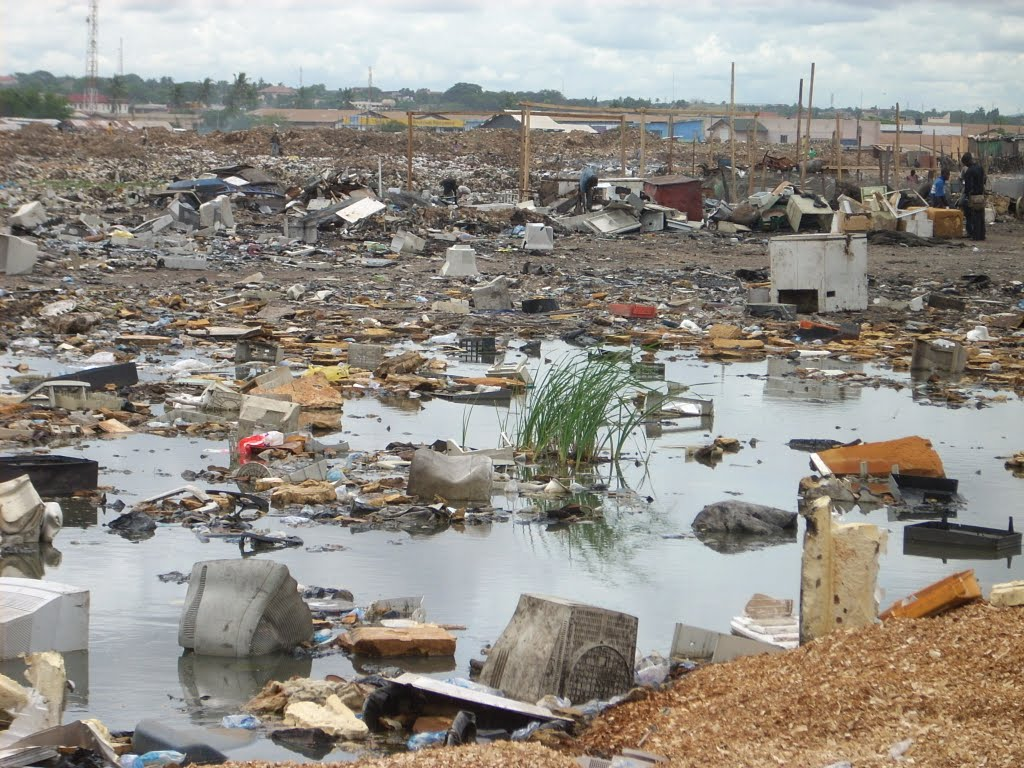
\includegraphics[width=0.5\textwidth]{../inputs/images/ewaste_jack_caravano.jpg}
  \caption{Foto do depósito de lixo eletrônico (\textit{e-waste}) situado no bairro 
           de Agbogbloshie em Acra. Autorizado por Jack Caravanos, 
           Professor da School of Public Health em Hunter College, CUNY
           Nova Iorque, Estado Unidos da América. \label{fig:ewaste}}
\end{figure}

%%%%
\subsection{Nima}

Nima é um dos bairros mais pobres de Acra e é formada de assentamentos não 
planejados compostos principalmente de migrantes das partes rurais e 
imigrantes de países vizinhos que buscam oportunidades de empregos na capital. 
As moradias são improvisadas e carece de sistema tratamento de esgoto, 
fornecimento de água potável e eletricidade. Além disso, muitas vias não são 
pavimentadas, causando o levantamento de poeira. 

%O meio de transporte dos trabalhadores para realizar o trajeto de suas casas a 
%zona industrial e comercial da cidade é usualmente feito por vans.

%A diversidade de Nima possui alta diversidade
%cultural e religiosa, e é conhecida por uma feira de comidas típicas 
%permanentemente instalada na região, (\textit{The Nima Market}).

As cozinhas dos moradores de Nima são instalações simples, adaptadas para o uso
de carvão e lenha como fonte de energia para o cozimento dos alimentos, 
podendo ser observadas nas imagens da figura \ref{fig:nima}.

\begin{figure}[H]
  \centering
    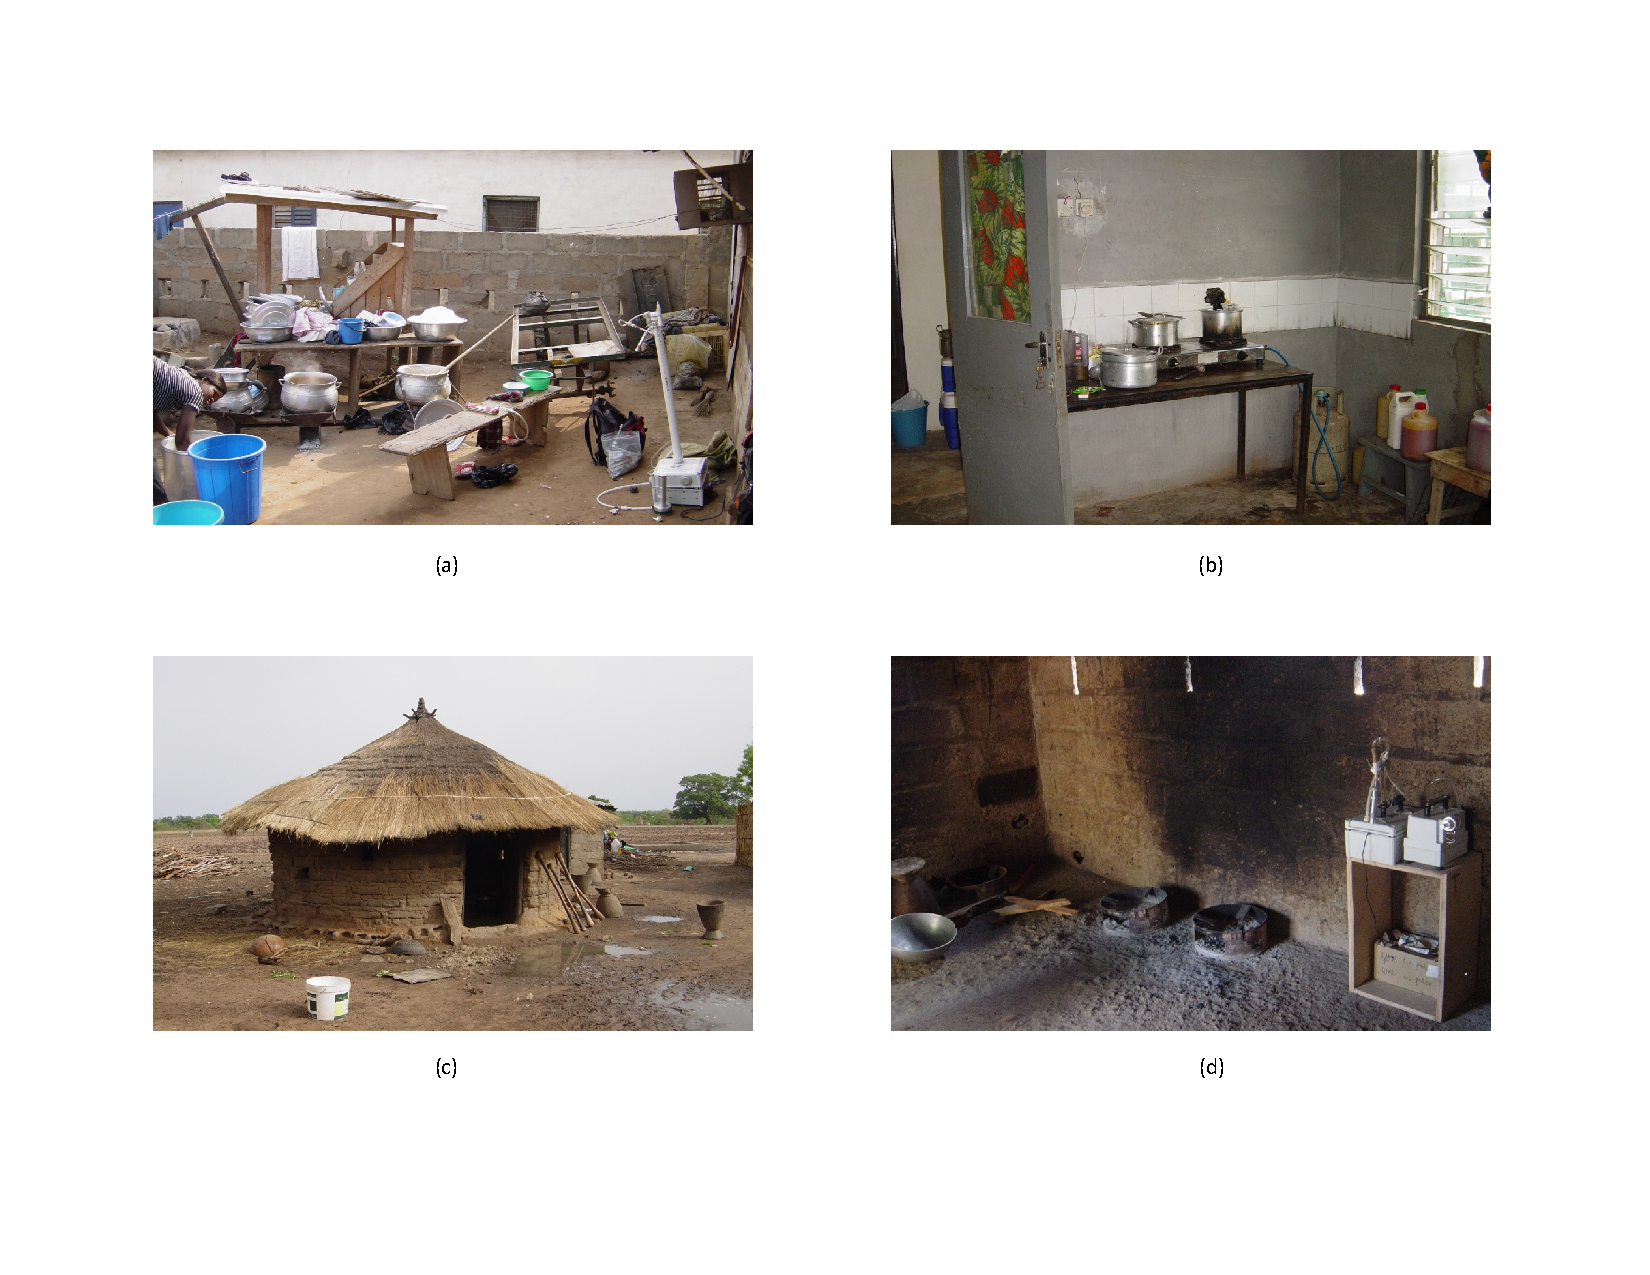
\includegraphics[width=0.7\textwidth]{../inputs/images/zheng/nima.pdf}
    \caption{Fotos de residências de Nima, por Raphael Arku \label{fig:nima}}
\end{figure}
